\section{Voraussetzungen}
Dieses Kapitel beschreib die Erstellung von Red-Book-kompatiblen Audio-CDs. Traverso verwendet \texttt{cdrdao} zum eigentlichen schreiben der CD, deshalb muss dieses Programm auf dem System installiert sein. \texttt{cdrdao} ist in allen gängigen Distributionen über die Software-Verwaltung erhältlich, was die Installation sehr einfach gestaltet. Auf Windows und Mac OS X installiert Traverso alle benötigten Zusatzprogramme selbständig, wodurch eine manuelle Installation entfällt. Benutzer dieser Plattformen können die folgende Anleitung überspringen.

\footnotesize
\begin{verbatim}
tux@linux:~$ cdrdao

Cdrdao version 1.2.2 - (C) Andreas Mueller <andreas@daneb.de>
  SCSI interface library - (C) Joerg Schilling
  Paranoia DAE library - (C) Monty

Check http://cdrdao.sourceforge.net/drives.html#dt for current 
driver tables.


Usage: cdrdao <command> [options] [toc-file]
command:
...
\end{verbatim}
\normalsize

Die Installation von \texttt{cdrdao} auf Linux-Systemen gestaltet sich in der Regel sehr einfach, da das Programm in allen aktuellen Distributionen enthalten ist und über den Paket-Manager installiert werden kann.

\section{Tracks und Marker}
Grundsätzlich gibt es zwei Möglichkeiten, die Tracks für eine CD festzulegen. Einerseits kann jedes Arbeitsblatt einen Track darstellen, oder die gesamte CD wird in einem Arbeitsblatt arrangiert, indem Trackmarker in der Zeitleiste platziert werden. Kombinationen dieser beiden Konzepte sind auch möglich. Betrachten wir sie aber einmal etwas genauer.

\subsection{Ein Arbeitsblatt als CD-Track}
Wie ihr vielleicht schon festgestellt habt, kann ein Projekt in Traverso mehrere Arbeitsblätter enthalten. Dies erlaubt, alle Lieder einer CD in einem Projekt zusammenzufassen, und trotzdem nur jeweils eines davon anzeigen zu lassen. Soll nun vom ganzen Projekt mit allen Arbeitsblättern eine CD gebrannt werden, achtet darauf, den Knopf ,,Alle Arbeitsblätter'' im CD-Export Dialog aktiviert zu haben. Dann wird jedes Arbeitsblatt von Position 00:00:00 bis zum Ende des letzten Audioclips einen CD-Track bilden.

\begin{figure}[t]
 \centering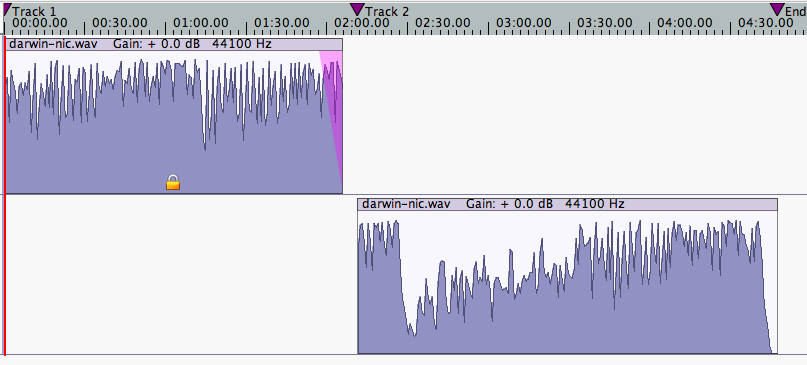
\includegraphics[width=\textwidth]{../images/markers01}
 \caption{Wenn eine CD in der Zeitachse arrangiert wird, werden die Tracks über Marker festgelegt. Bei Position 00:00:00 und am Ende des Projektes müssen jeweils Marker vorhanden sein.}
 \label{fig_markers01}
\end{figure}

\subsection{CD in der Zeitachse}
Manchmal sollen die Übergänge zwischen den CD-Tracks speziell bearbeitet werden, zum Beispiel indem man etwas Stille einfügt bevor das nächste Stück beginnt, oder indem man den Übergang überblendet. In solchen Fällen ist es einfacher, die CD in einem Arbeitsblatt zusammenzustellen, und die Tracks durch Markierungen in der Zeitachse festzulegen. Ein Beispiel dazu ist in \FigT~\ref{fig_markers01} abgebildet. Öffnet dazu ein Projekt mit nur zwei Audioclips, oder erstellt ein solches. Clip 1 soll als Track 1 auf die CD geschrieben werden, Clip 2 entsprechend als Track 2. Positioniert Clip 1 an Position 00:00:00, und Clip 2 hinter Clip 1 mit einer kleinen Lücke dazwischen, so dass der Übergang angenehm klingt. Haltet nun den Mauszeiger über die Lücke zwischen den Clips und drückt \sact{M}. In der Zeitachse wird an der Stelle ein kleines Dreieck eingefügt, ebenso bei Position 00:00:00 und am Ende des zweiten Clips. Letzteres ist mit ,,End'' beschriftet, und es markiert das Ende der CD. Falls ihr ein Hall-Plugin aktiviert habt, müsst ihr das Ende etwas nach hinten schieben, da die Hallfahne unter Umständen etwas über das Ende des Clips hinaus nachklingt.

Diese Dreiecke sind Marker, und sie können frei verschoben, hinzugefügt oder gelöscht werden (\sact{Q} auf der Zeitachse listet alle Aktionen auf). Es ist jedoch möglich, Arrangements zu erstellen die keinen Sinn ergeben, zum Beispiel indem man keinen Marker am Anfang oder Ende des Projektes einfügt. In diesem Fall versucht Traverso, eine sinnvolle Lösung zu finden und fügt die notwendigen Marker automatisch beim Brennen hinzu. Traverso unterstützt CD-Text, der in einem speziellen Dialog (,,Ansicht $\rightarrow$ Marker-Dialog'', \FigT~\ref{fig_marker-editor}) bearbeitet werden kann. Aus diesem Dialog kann das Inhaltsverzeichnis als HTML-Datei exportiert werden. CD-Textfelder welche die gesamte CD betreffen können im Dialog ,,Projekt $\rightarrow$ Projektmanager'' im Karteireiter ,,CD-Text'' bearbeitet werden.

\begin{figure}[ht]
 \centering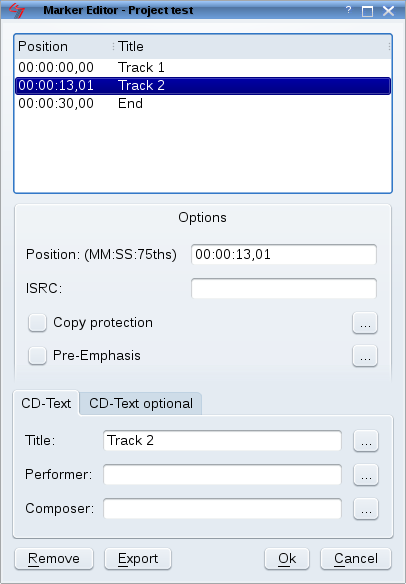
\includegraphics[width=0.45\textwidth]{../images/marker-editor}
 \caption{Der Marker-Dialog ,,Ansicht $\rightarrow$ Marker-Dialog'' erlaubt die Eingabe von CD-Text, das Verschieben und Umbenennen von Markern, und den Export des Inhaltsverzeichnisses als HTML-Datei.}
 \label{fig_marker-editor}
\end{figure}

Ist die CD fertig arrangiert, drückt \sact{F8} um CD-Brenndialog zu öffnen (\FigB~\ref{fig_exportdlg}). Nun müsst ihr entscheiden, ob nur das aktuelle Arbeitsblatt (mit Markern als CD-Tracks) oder das ganze Projekt (jedes Arbeitsblatt stellt einen CD-Track dar) gebrannt werden soll. Aktiviert ihr die Option ,,Nur in Datei exportieren'', wird das CD-Abbild auf die Festplatte geschrieben, jedoch nicht auf die CD. Das Abbild kann später mit \texttt{cdrdao} auf CD geschrieben werden.

Wichtig für OS X-Benutzer: Die CD-Brennfunktion befindet sich noch in einem frühen Entwicklungsstadium. Es können mehrere Brenngeräte ausgewählt werden: IODVDServices, IODVDServices/2, IOCompactDiscServices, IOCompactDiscServices/2. Diese Einträge wurden fest programmiert, und es kann sein, dass nicht alle Geräte auch wirklich vorhanden sind. IOCompactDiscServices sollte nur verwendet werden, wenn das Laufwerk noch keine DVD-Leseunterstützung bietet. In allen anderen Fällen sollten IODVDServices oder IODVDServices/2 ausgewählt werden, um das erste bzw. zweite DVD-Laufwerk anzusprechen. Normalerweise ist IODVDServices die beste Wahl.

\begin{figure}[t]
 \centering
 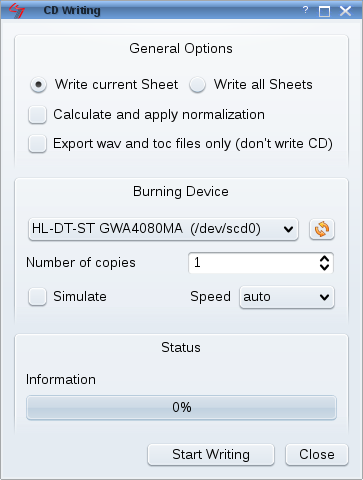
\includegraphics[width=0.35\textwidth]{../images/exportdlg}\qquad
 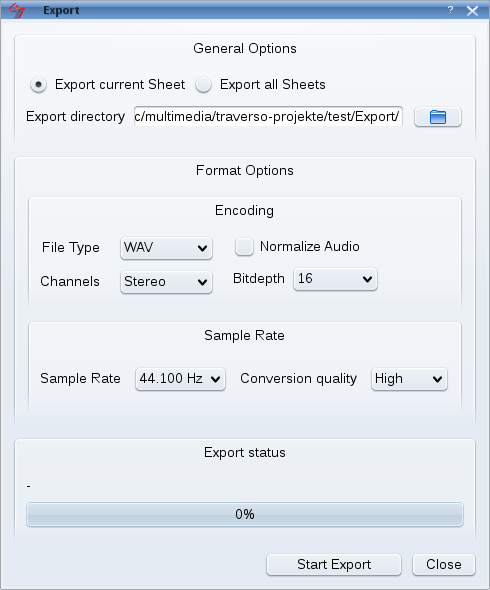
\includegraphics[width=0.45\textwidth]{../images/exportdlg1}
 \caption{\sact{F8} öffnet einen Dialog, mit dem entweder das aktuelle Arbeitsblatt oder das ganze Projekt auf CD gebrannt werden kann (links). Mit \sact{F9} öffnet man einen Dialog, mit dem das Projekt oder Arbeitsblatt in eine Audiodatei exportiert werden kann.}
 \label{fig_exportdlg}
\end{figure}

Um das Projekt in eine Audiodatei zu exportieren drückt \sact{F9} oder wählt ,,Projekt $\rightarrow$ Export\dots''. Für den Dateiexport stehen mehrere Dateiformate zur Verfügung, darunter WAVE, WavPack, FLAC, Ogg/Vorbis und MP3. Das gebräuchlichste ist WAVE, das in verschiedenen Bittiefen exportiert werden kann. Wählt 16~bit wenn ihr die Datei später auf CD brennen wollt, und 32~bit wenn die Datei noch weiter bearbeitet werden soll. Zur Archivierung wählt FLAC oder WavPack um die Dateien ohne Qualitätsverlust zu komprimieren. Sollten nicht alle Formate verfügbar sein, wurde die Unterstützung bei der Kompilation von Traverso deaktiviert. Einige Distributionen unterstützen aus rechtlichen Gründen keine patentierten Formate. In diesem Fall muss man entweder damit leben, oder Traverso mit der entsprechenden Unterstützung neu kompilieren.
